\documentclass{beamer}
 
\usepackage[utf8]{inputenc} 
\usepackage[T1]{fontenc}
\usepackage{lmodern}
\usepackage{graphicx}
\usepackage[french]{babel}
\usepackage{animate}
\usepackage{movie15}
\usepackage{relsize}
 
\usetheme{Frankfurt}

\title[Soutenance]{Soutenance du TPA}
\subtitle[\ldots]{Rapport}
\author[FTL]{Simon \textsc{Bihel}, Sebastien \textsc{Gamblin}, Josselin \textsc{Gueneron}, Julien \textsc{Pezant}, Paul \textsc{Lemenager}}
\institute[UCBN]{UCBN L2 Informatique Semestre 2}
\date{\today}
 
\begin{document}
\begin{frame}
	\maketitle
\end{frame}

\begin{frame}
	\frametitle{Plan}
	\tableofcontents
\end{frame}

\section{Introduction}
\begin{frame}
	\frametitle{Présentation du jeu}
	%\subsection{Présentation du jeu}
	\begin{center}
		\Large{\textit{FTL : Faster Than Light}, Subset Games.}

		RTS, roguelike.
	\end{center}
	\begin{figure}[H]
		\centering
		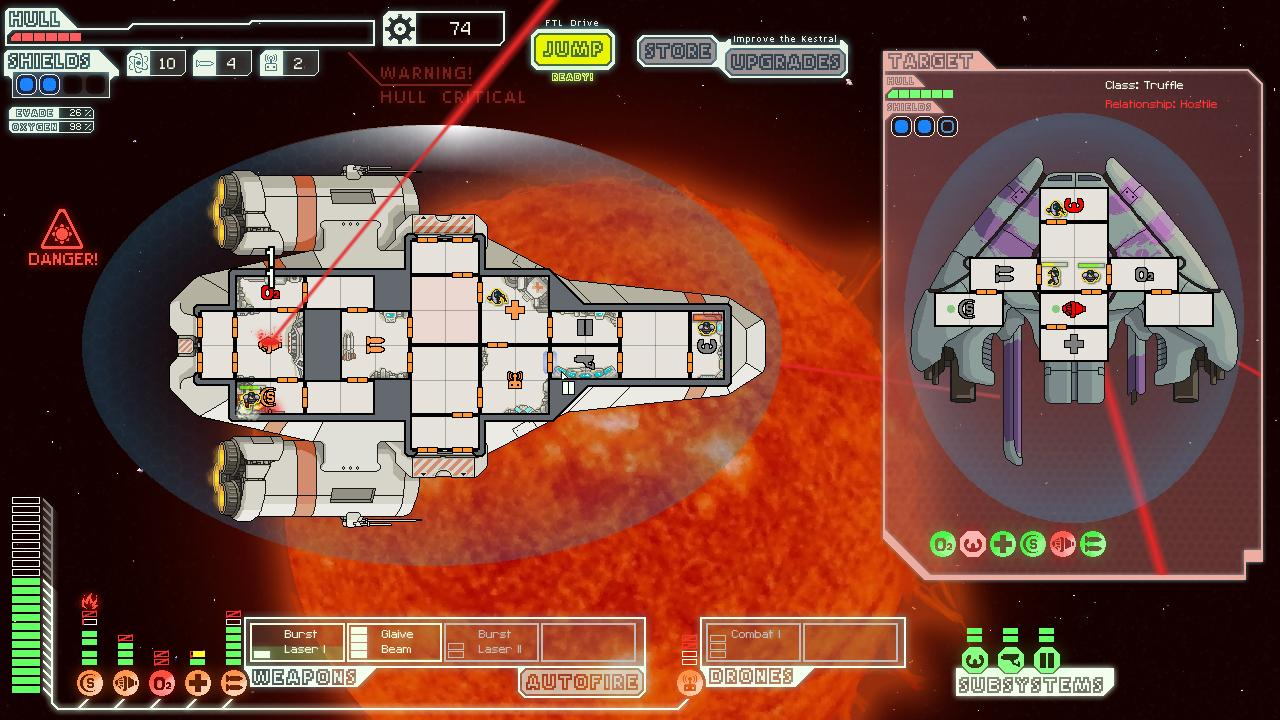
\includegraphics[width=0.7\linewidth]{screen.jpg}
	\end{figure}
	
\end{frame}

\begin{frame}
	%\subsection{Présentation du projet}
	\frametitle{Présentation du projet}
	\begin{itemize}
		\item Réalisation d'un programme permettant la modélisation de vaisseaux de FTL afin de les optimiser au mieux
		\item La modélisation des vaisseaux ainsi que la simulation de combats ont été réalisés lors du premier semestre
		\item Le but du second semestre est de faire un programme déterminant le meilleur vaisseau pour un coût maximal donné. C'est-à-dire :
		\begin{itemize}
			\item faire un générateur de vaisseaux selon un coût donné ;
			\item faire un algorithme déterminant le meilleur vaisseau.
		\end{itemize}
	\end{itemize}
	
\end{frame}

\section{Le moteur de combats}
\subsection{Rappels sur le moteur de combats}
\begin{frame}
	\frametitle{Rappel sur le moteur de combats}
	\begin{itemize}
		\item Tour par tour
		\item Cooldowns et phases d'attaque gérés séparément
		\item Deux représentations/stockages : la représentation des vaisseaux de base et la représentation des vaisseaux personnalisés
	\end{itemize}
	\begin{figure}
		\caption{Exemple de vaisseau personnalisé}
		\vspace*{-5cm} 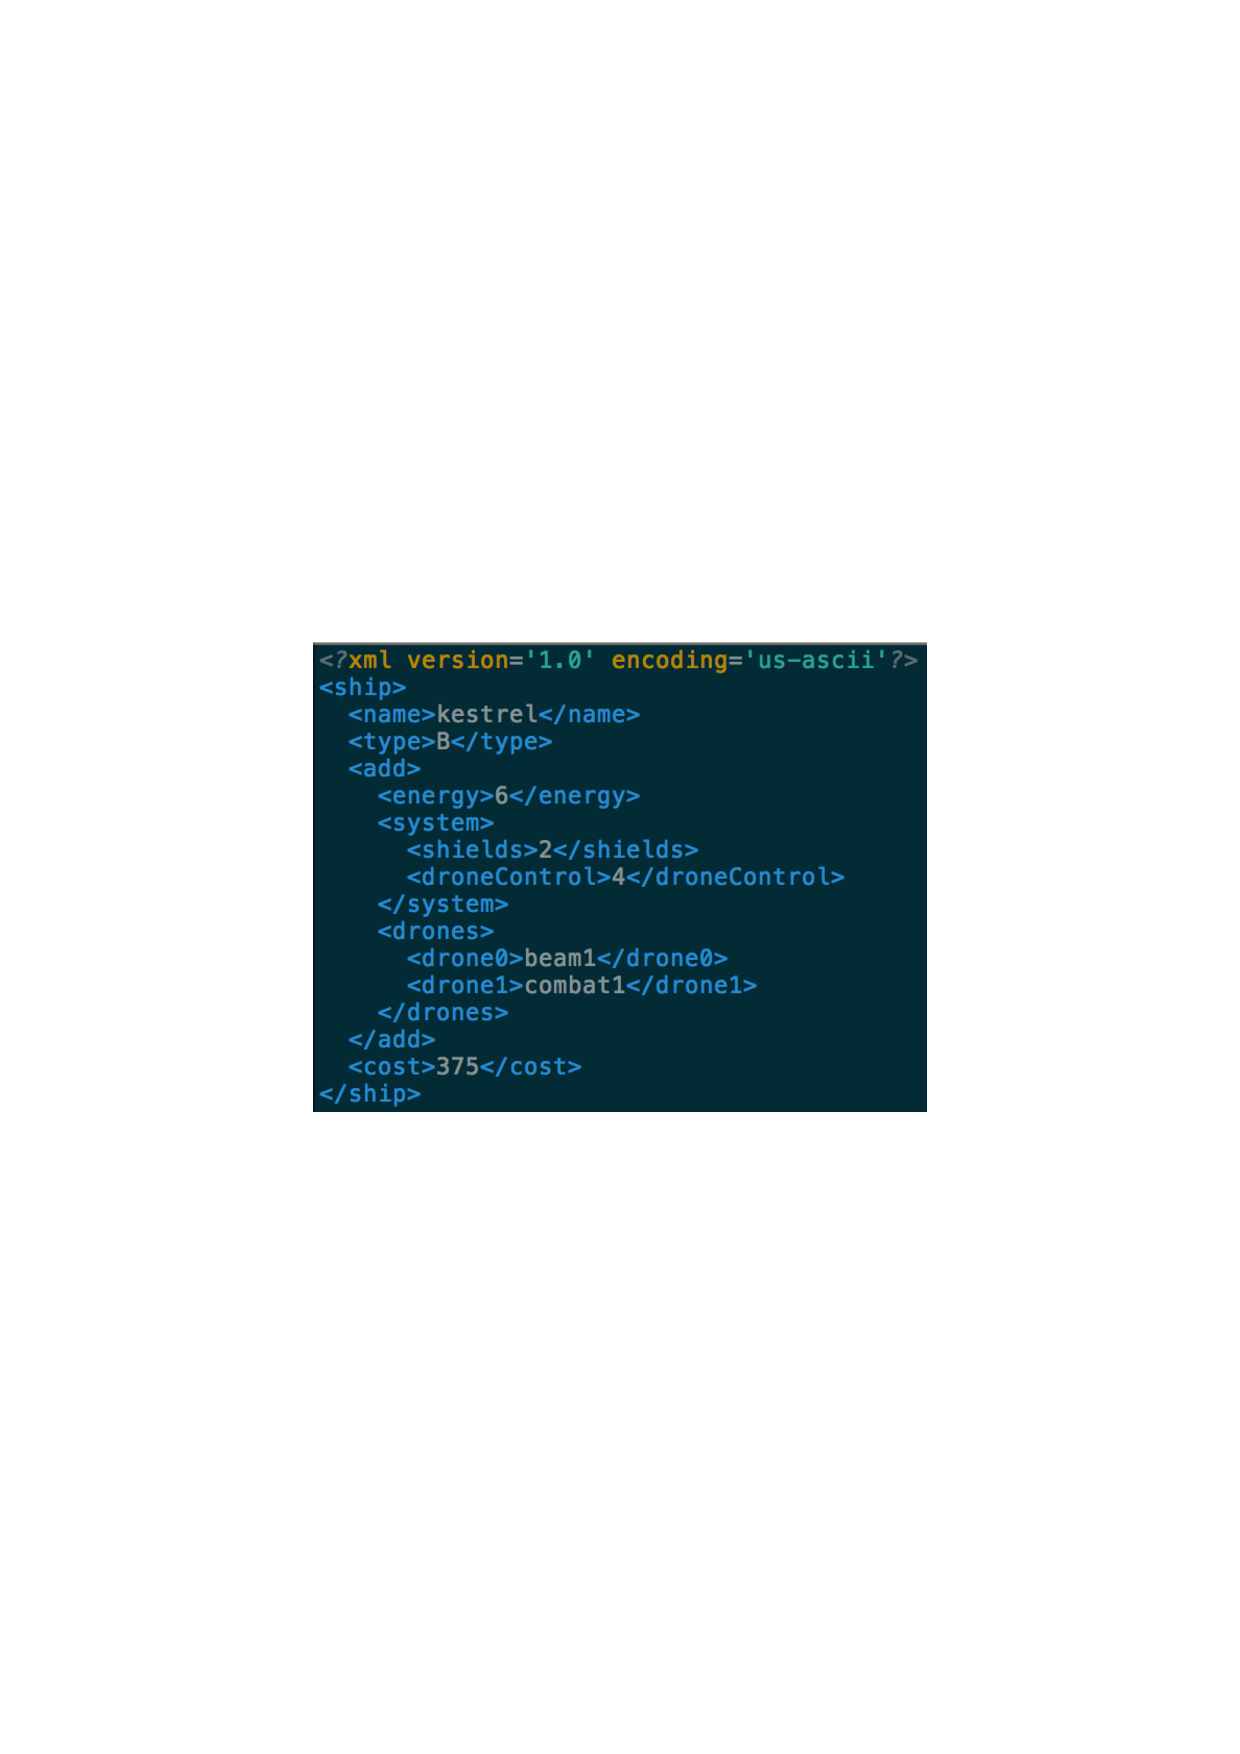
\includegraphics[height=1.55\textheight]{shipPersonnalizedExample.pdf}
	\end{figure}
	
\end{frame}

\subsection{Ajouts au moteur de combats}
\begin{frame}
	\frametitle{Ajouts au moteur de combats}
	\begin{itemize}
		\item Discrétisation des évènements avec une liste d'évènements pour les phases d'attaque et une liste pour les cooldowns
		\item Nouvelle représentation graphique avec tkinter
		\item Tournois entre plusieurs vaisseaux
		\item Affichage HTML des résultats d'un tournois
	\end{itemize}
	\vspace*{-3.3cm} 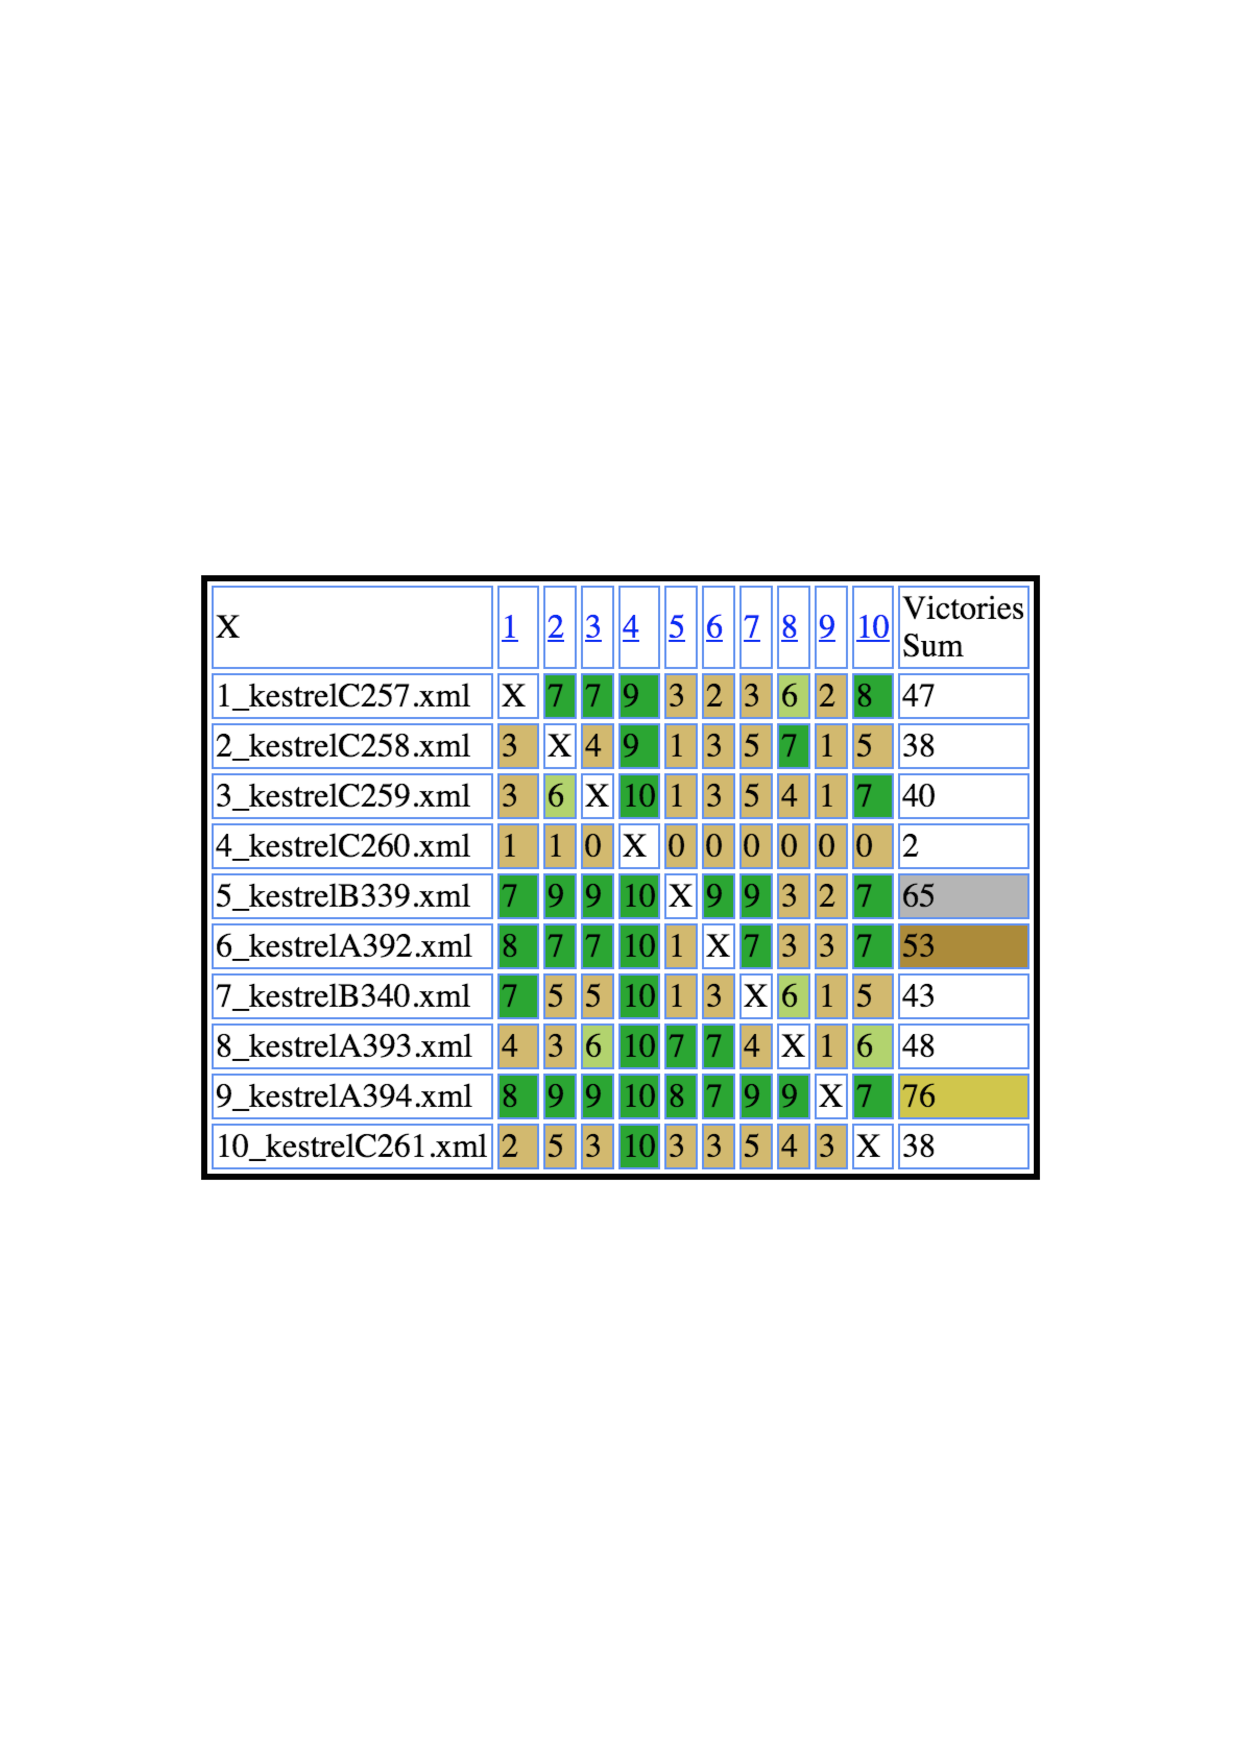
\includegraphics[scale=0.4]{tournamentResultExample.pdf}
	
\end{frame}

\subsection{Affichage graphique}
\begin{frame}
	\frametitle{Affichage graphique}
	\begin{figure}[H]
		\centering
		\hspace*{-1cm}
		%\includemovie{1cm}{1cm}{finalgif3.gif}
		%\includegraphics[width=0.75\linewidth]{finalgif3.gif}
		\animategraphics[scale=0.299]{2}{finalgif3-}{0}{22}
	\end{figure}
\end{frame}

\section{Recherche du meilleur vaisseau}
\begin{frame}
	\frametitle{Recherche du meilleur vaisseau}
	On appellera "meilleur vaisseau" celui qui gagne plus de combats que les autres. 

	Différents éléments dans le programme.
	\begin{enumerate}
		\item Un générateur de vaisseaux.
		\item Un algorithme génétique.
		\item Un système expert.
	\end{enumerate}
\end{frame}

\subsection{Générateur aléatoire de vaisseaux}
\begin{frame}
	\frametitle{Générateur aléatoire de vaisseaux}
	\begin{columns}[T]
		\begin{column}{.5\textwidth}
			\vspace*{-0.4cm} 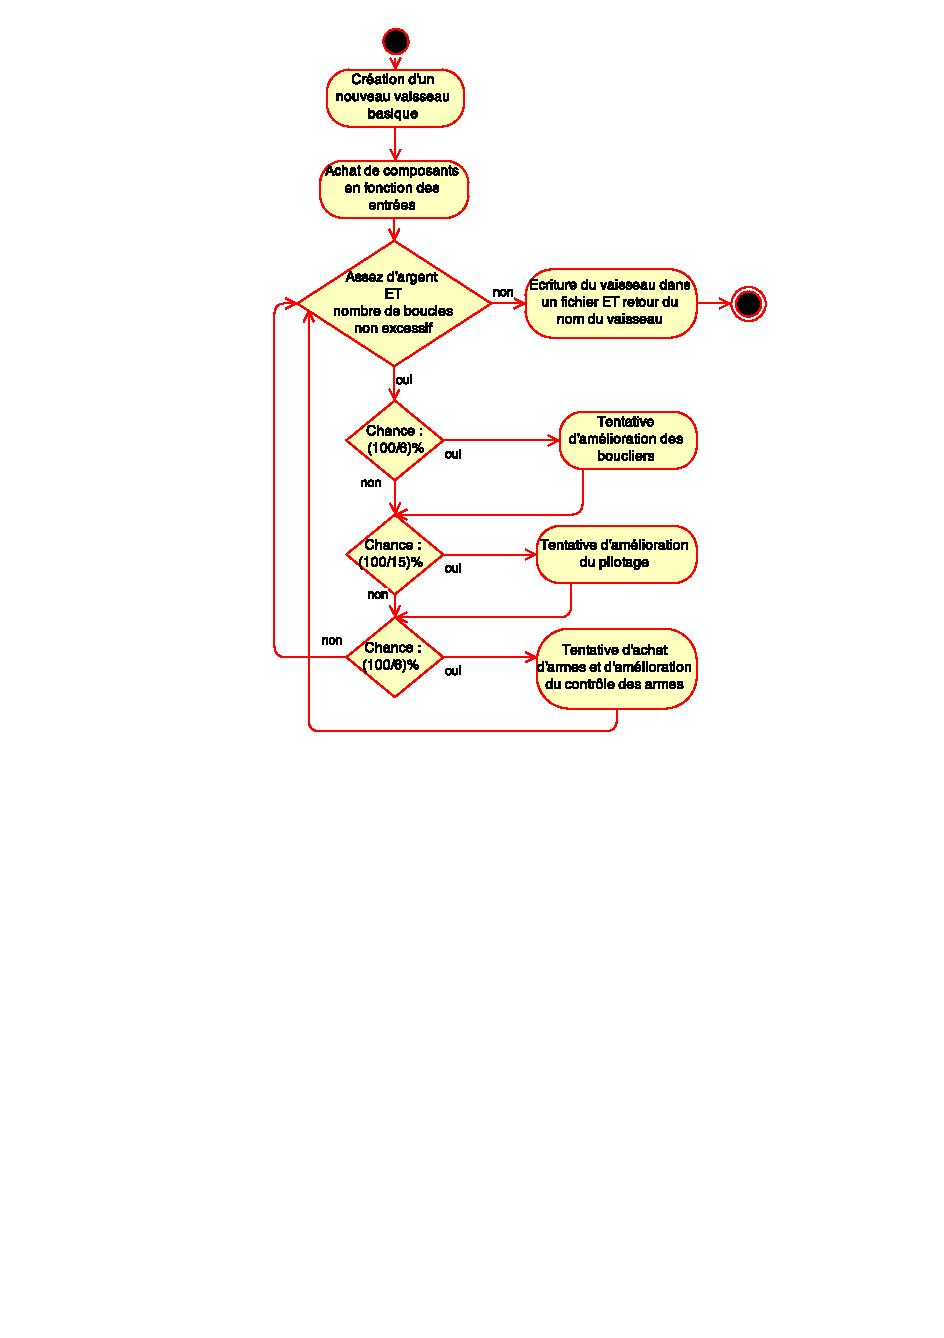
\includegraphics[height=0.91\textheight]{randomGeneratorCut.pdf} \hspace*{\fill}
		\end{column}
		\begin{column}{.6\textwidth}
			\begin{itemize}
				\item Schéma tronqué (il n'y a pas toutes les types d'équipement)
			\end{itemize}
		\end{column}
	\end{columns}
\end{frame}

\begin{frame}
	\frametitle{Générateur aléatoire : les moteurs}
	\begin{figure}[H]
		\centering
		\vspace*{-0.35cm} 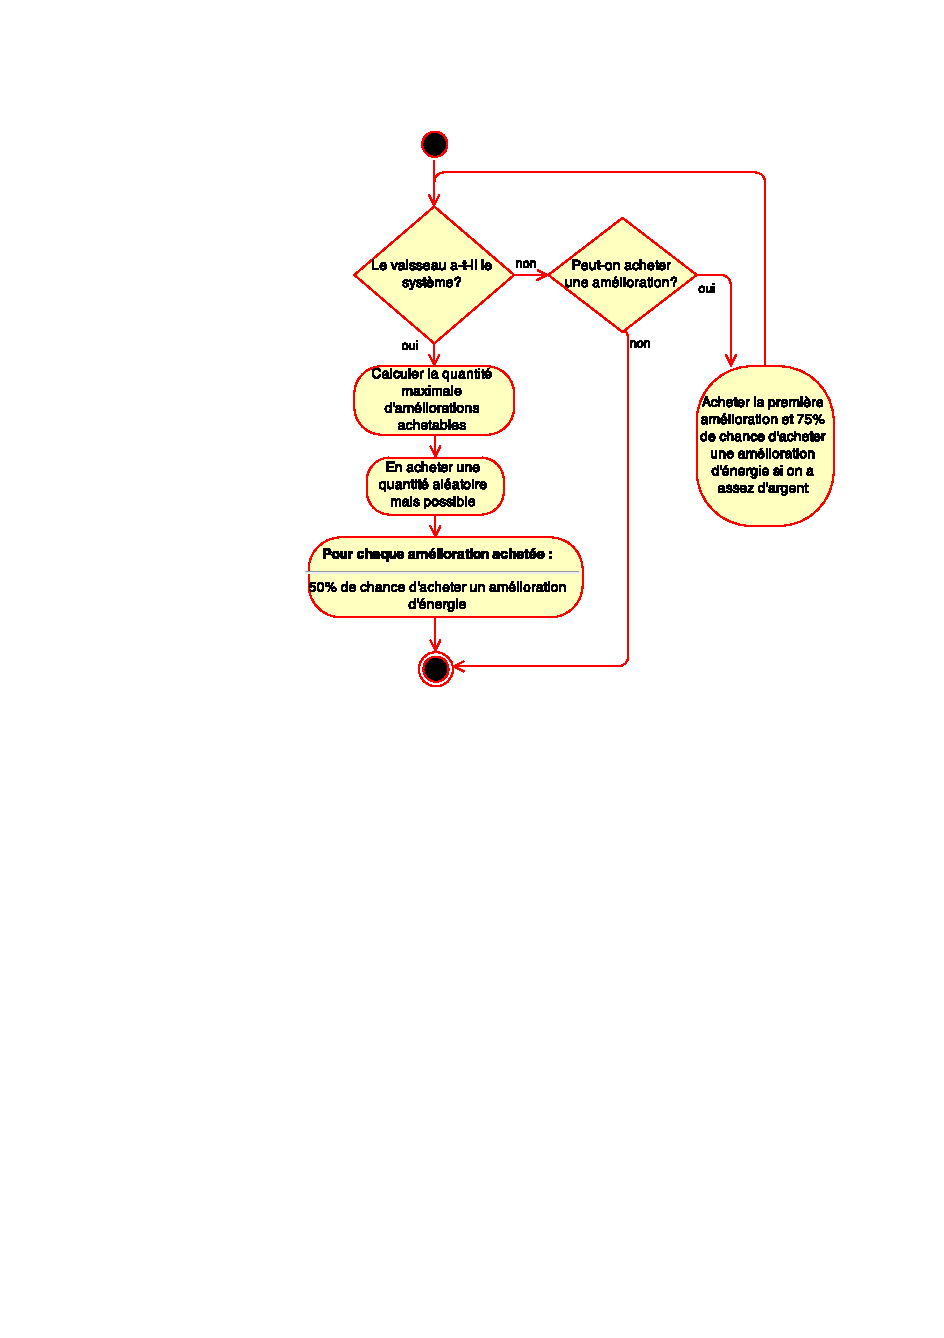
\includegraphics[height=0.89\textheight]{randomGeneratorExample.pdf}
	\end{figure}
\end{frame}

\subsection{Algorithme génétique}
\begin{frame}		
	\frametitle{Algorithme génétique}
	\begin{figure}[H]
		\centering
		\vspace*{-0.45cm} 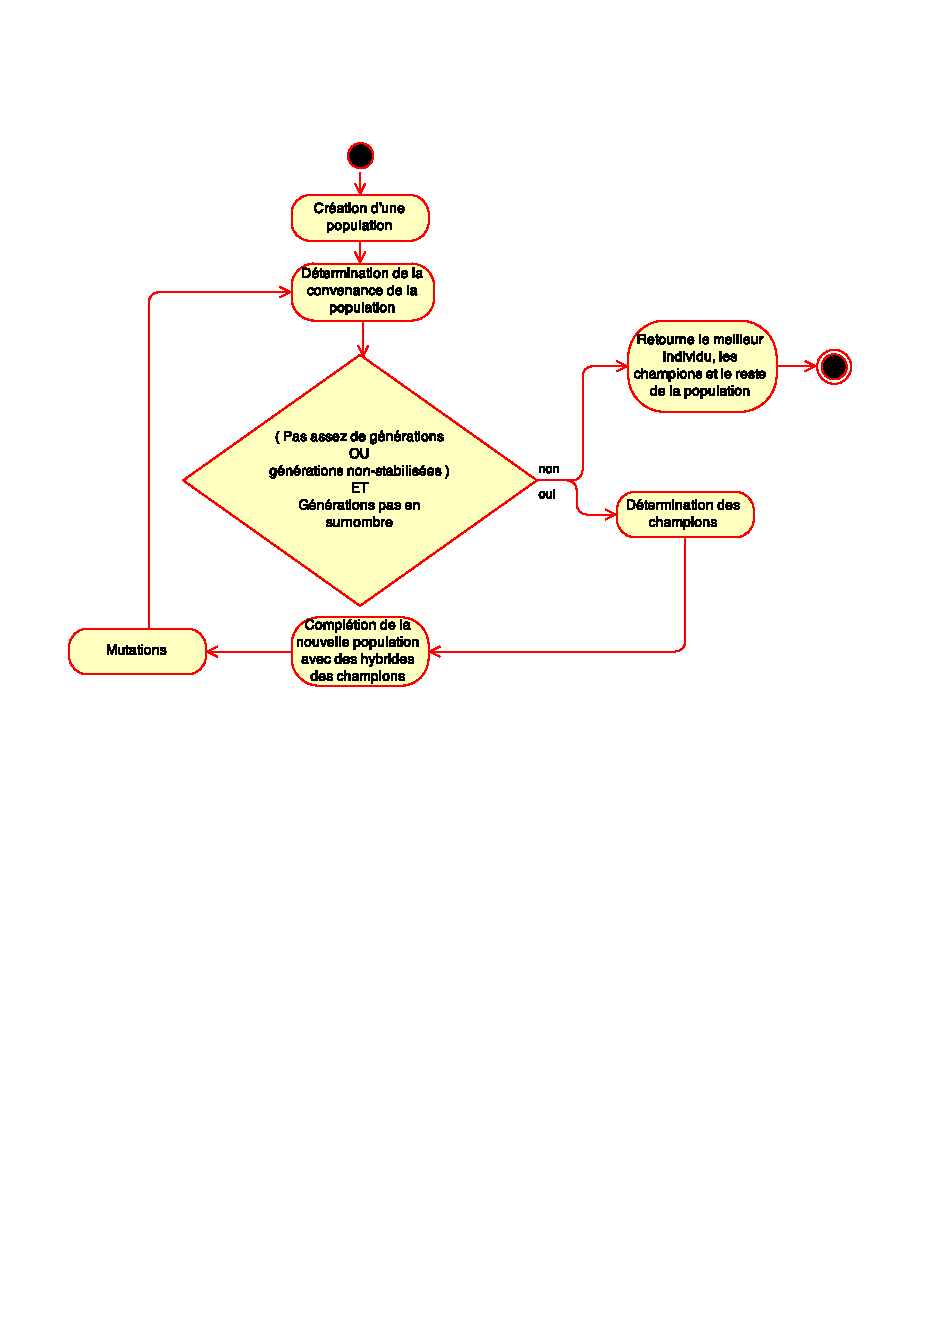
\includegraphics[height=0.85\textheight]{geneticAlgorithm.pdf}
	\end{figure}
\end{frame}

\subsection{Data Mining}
\begin{frame}
	\frametitle{Data Mining}
	\begin{itemize}
		\item Utilisation du programme \textit{Linear time Closed itemset Miner} de Takeaki Uno
		\item Chaque ligne représente l'équipement d'un vaisseau
		\item Chaque pièce d'équipement est représenté par un entier (e.g. niveau d'un système entre 31 et 179)
		\item Pour chaque niveau d'amélioration, les niveaux inférieurs sont aussi dans la ligne (e.g. energy1 energy2 energy3)
	\end{itemize}
\end{frame}

\subsection{Algorithme final d'optimisation}
\begin{frame}
	\frametitle{Algorithme final d'optimisation}
	\begin{columns}[T]
		\begin{column}{.25\textwidth}
			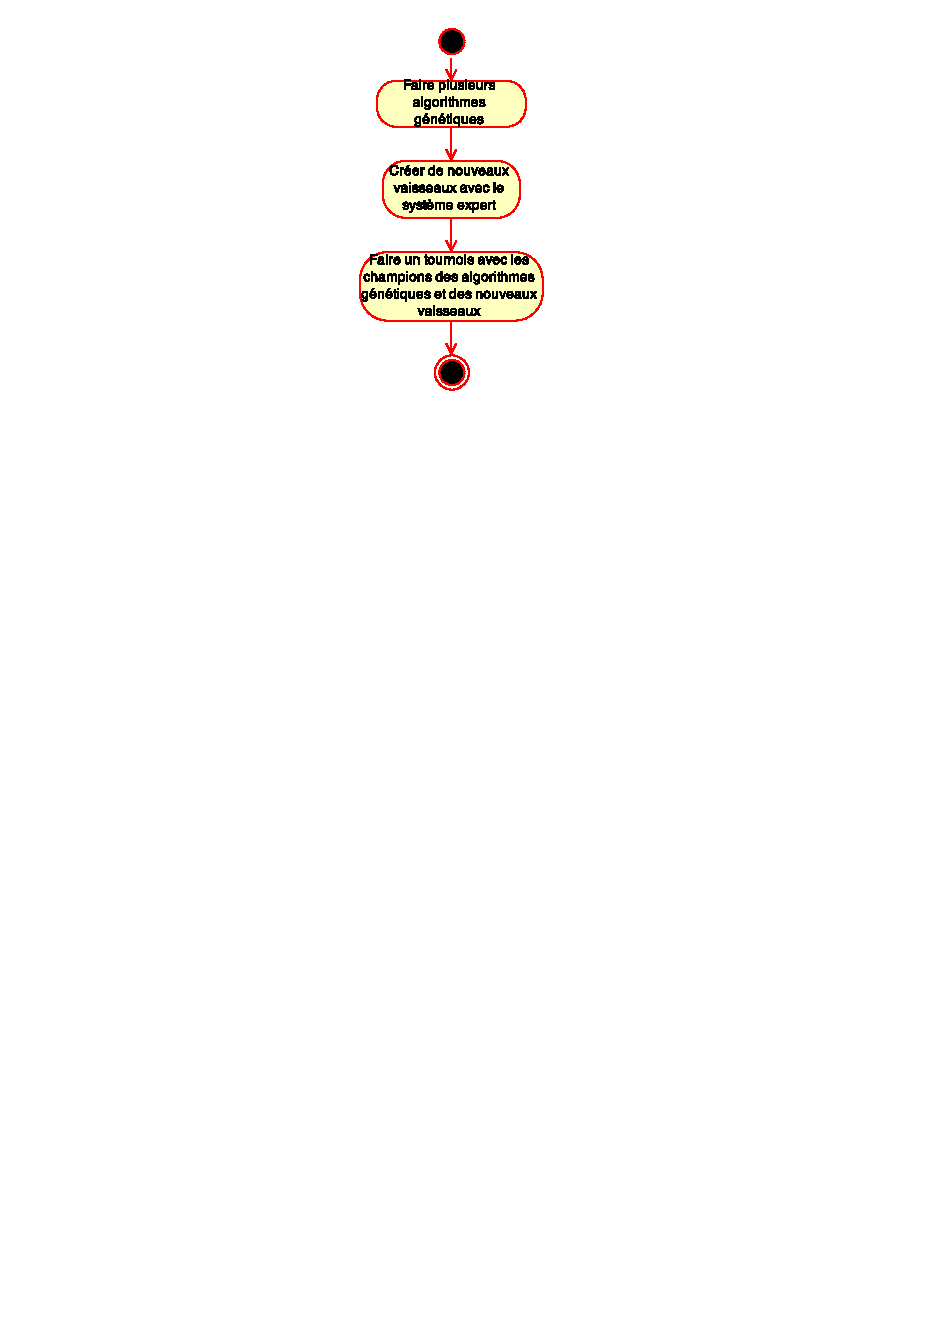
\includegraphics[height=0.75\textheight]{finalAlgorithm.pdf} \hspace*{\fill}
		\end{column}
		\begin{column}{.75\textwidth}
			Caractéristique : ensemble de pièces d'équipement
			\center{Le système expert}
			\begin{itemize}
				\item Création de vaisseaux qui ont les caractéristiques propres aux champions
				\item Taux de croissance d'une caractéristique : $\rho (P) = \mathlarger{\frac{\ \ \frac{S_{+}}{D_{+}} \ \ }{\ \ \frac{S_{-}}{D_{-}} \ \ }}$, $S_{\pm}$ le nombre d'occurences et $D_{\pm}$ le nombre de vaisseaux
				\item Taux de confiance : $\mbox{conf} = \mathlarger{\frac{\rho (P)}{\rho (P)+1}}$
			\end{itemize}
		\end{column}
	\end{columns}
\end{frame}

\section{Réalisation}
\subsection{Les modules}
\begin{frame}
	\frametitle{Les modules}
	\hspace*{-1cm} \vspace*{3cm} 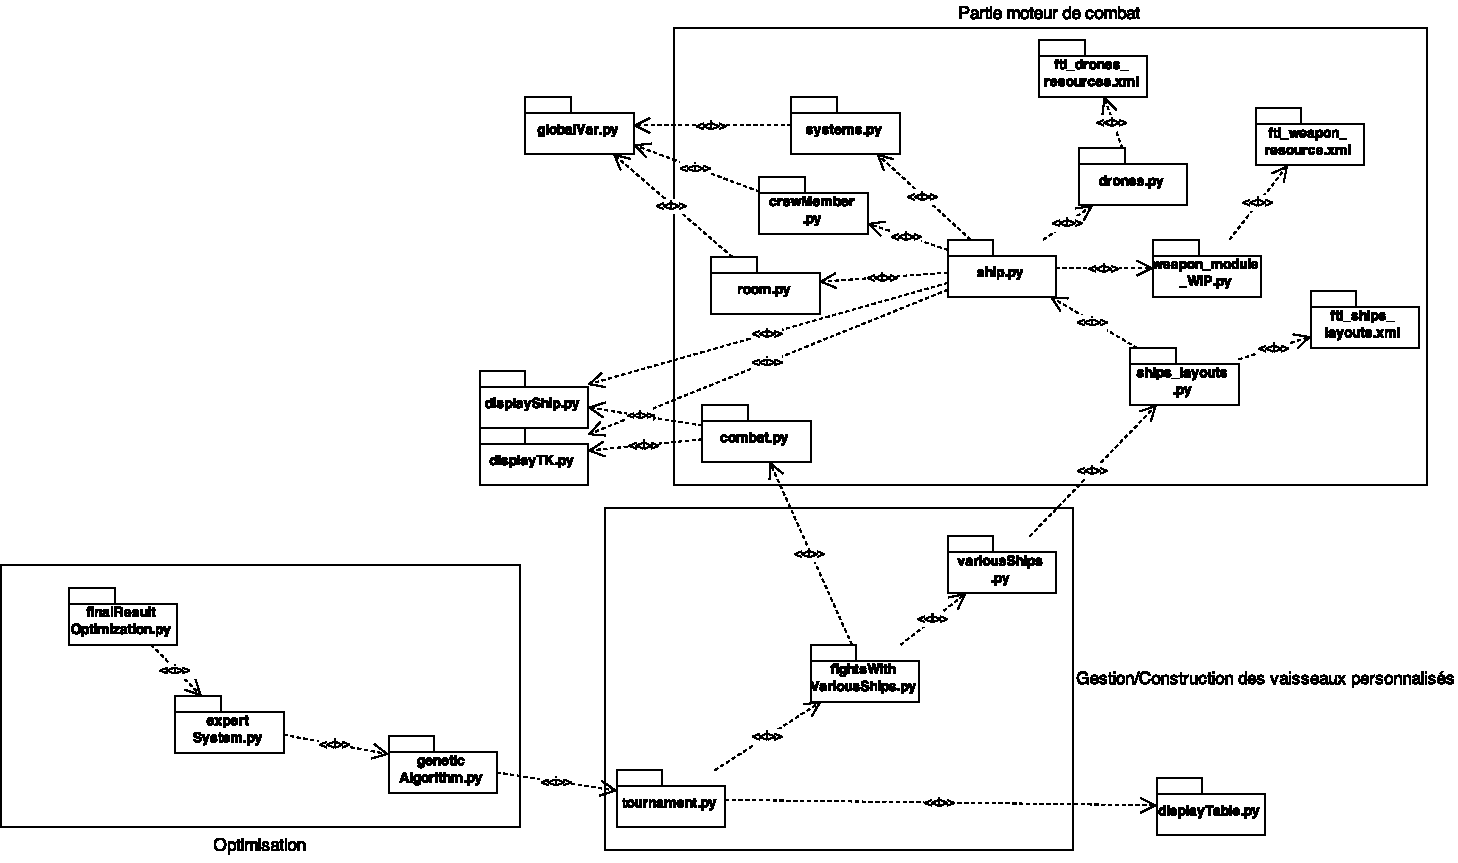
\includegraphics[height=0.84\textheight]{packageDiagramHorizontal.pdf}
\end{frame}

\subsection{Failles du programme}
\begin{frame}
	\frametitle{Failles du programme}
	\begin{itemize}
		\item Incomplétude du moteur de combats et du générateur aléatoire
		\item \textit{Metagame} dans les algorithmes génétiques
		\item Les mauvais vaisseaux et les bons sont plus ou moins similaires en fonction de la fin par stabilisation des algorithmes génétiques
	\end{itemize}
\end{frame}

\section{Conclusion}
\begin{frame}
	\frametitle{Conclusion}
	\begin{itemize}
		\item Objectifs atteints
		\item Futures pistes :
			\begin{itemize}
				\item déplacements de l'équipage ;
				\item optimisation du temps mis par les tournois.
			\end{itemize}
	\end{itemize}
\end{frame}

\end{document}

